\subsubsection{PSoC\_Master Klassen}
\begin{figure}[h]
\centering 
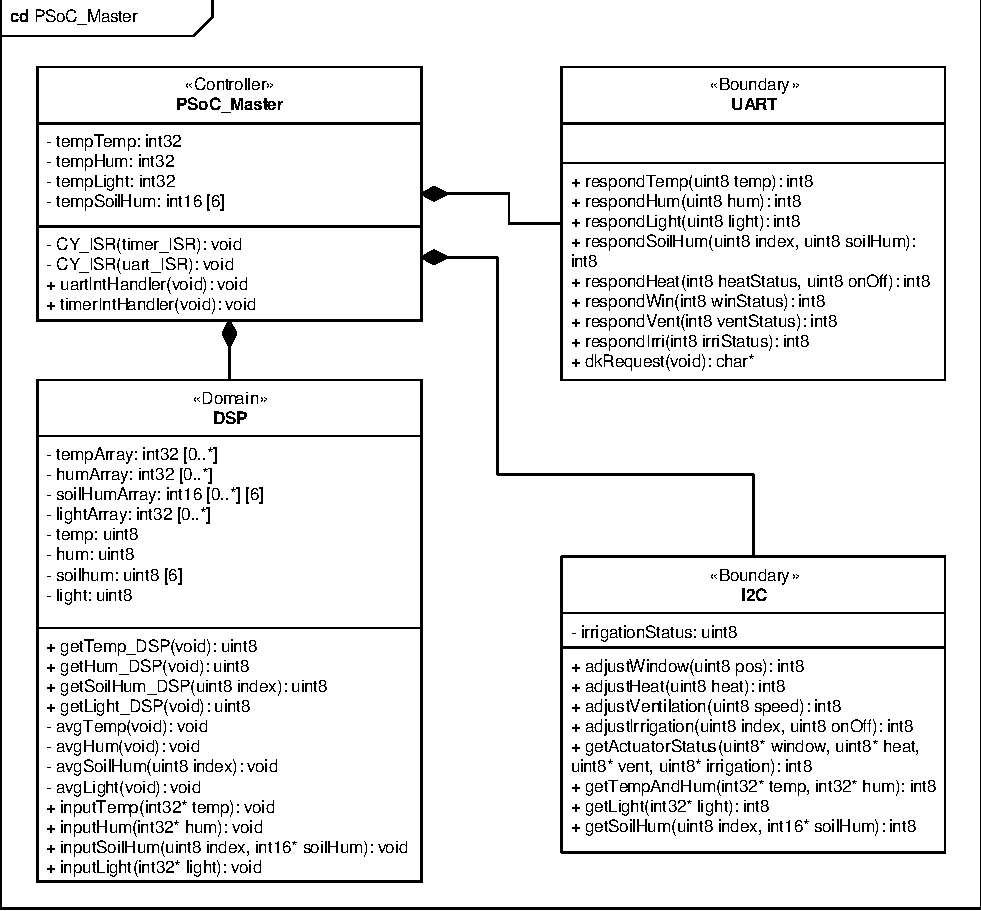
\includegraphics[width=\textwidth * 2/5, trim=15 282 269 31, clip=true] {../fig/cd_PSoC_master.pdf}
\caption{PSoC\_Master klassen.}
\label{fig:Master_PSoC_klasse}
\end{figure}

På Figur \ref{fig:Master_PSoC_klasse} ses et diagram for PSoC\_Master klassen.
Formålet og tanken bag klassen er, at denne skal styre al funktionalitet i PSoC Master blokken.
Som udgangspunkt var det tænkt, at al funktionalitet skulle ligge i de to interrupt service rutiner (\texttt{timer\_ISR} og \texttt{uart\_ISR}). 
Dette viste sig sidenhen at være uhensigtsmæssigt, da der ofte opstod konflikter mellem de to interrupt service rutiner.
Der blev derfor lavet to yderligere metoder, nemlig \texttt{uartIntHandler()} og \texttt{timerIntHandler()} til at håndtere funktionaliteten for hhv. UART og timer.
Dette viste sig at løse en del af problemerne.

Der er senere erfaret, at samhørigheden kunne være større ved at lade interrupt service rutinerne ligge i deres respektive klasser, da de er tæt knyttet til hardwaren.
Dog blev de lagt i PSoC\_Master klassen, da de oprindeligt var tiltænkt at også indeholde al funktionaliteten.